% Author: Izaak Neutelings (October 2021)
% Inspiration
%   "Very special relativity - An illustrated guide", Sander Bais (2007)
%   http://people.uncw.edu/hermanr/GR/Minkowski/Minkowski.pdf
\documentclass[border=3pt,tikz]{standalone}
\usepackage{amsmath} % for \text
\usepackage{etoolbox} % ifthen
\usepackage[outline]{contour} % glow around text
\usetikzlibrary{calc} % for adding up coordinates
\usetikzlibrary{decorations.markings,decorations.pathmorphing}
\usetikzlibrary{angles,quotes} % for pic (angle labels)
\usetikzlibrary{arrows.meta} % for arrow size
\usepackage{xfp} % higher precision (16 digits?)
\contourlength{1.1pt}

\tikzset{>=latex} % for LaTeX arrow head
\colorlet{myred}{red!85!black}
\colorlet{mydarkred}{red!55!black}
\colorlet{mylightred}{red!85!black!12}
\colorlet{myfieldred}{mydarkred!5} % for S' background
\colorlet{myredhighlight}{myred!20} % highlights simultaneity in ladder paradox
\colorlet{myblue}{blue!80!black}
\colorlet{mydarkblue}{blue!50!black}
\colorlet{mylightblue}{blue!50!black!30}
\colorlet{mylightblue2}{myblue!10}
\colorlet{mygreen}{green!80!black}
\colorlet{mypurple}{blue!40!red!80!black}
\colorlet{mydarkgreen}{green!50!black}
\colorlet{mydarkpurple}{blue!40!red!50!black}
\colorlet{myorange}{orange!40!yellow!95!black}
\colorlet{mydarkorange}{orange!40!yellow!85!black}
\colorlet{mybrown}{brown!20!orange!90!black}
\colorlet{mydarkbrown}{brown!20!orange!55!black}
\colorlet{mypurplehighlight}{mydarkpurple!20} % highlights simultaneity in ladder paradox
\tikzstyle{world line}=[myblue!40,line width=0.3]
\tikzstyle{world line t}=[mypurple!50!myblue!40,line width=0.3]
\tikzstyle{world line'}=[mydarkred!40,line width=0.3]
\tikzstyle{mysmallarr}=[-{Latex[length=3,width=2]},thin]
\tikzstyle{mydashed}=[dash pattern=on 3 off 3]
\tikzstyle{rod}=[mydarkbrown,draw=mydarkbrown,double=mybrown,double distance=2pt,
                 line width=0.2,line cap=round,shorten >=1pt,shorten <=1pt]
%\tikzstyle{rod'}=[rod,draw=mydarkbrown!80!red!85,double=mybrown!80!red!85]
\tikzstyle{vector}=[->,line width=1,line cap=round]
\tikzstyle{vector'}=[vector,shorten >=1.2]
\tikzstyle{particle}=[mygreen,line width=0.9]
\tikzstyle{photon}=[-{Latex[length=5,width=4]},myorange,line width=0.8,decorate,
                    decoration={snake,amplitude=1.0,segment length=5,post length=5}]

\def\tick#1#2{\draw[thick] (#1) ++ (#2:0.06) --++ (#2-180:0.12)}
\def\tickp#1#2{\draw[thick,mydarkred] (#1) ++ (#2:0.06) --++ (#2-180:0.12)}
\def\Nsamples{100} % number samples in plot

\begin{document}

% SPACETIME DIAGRAM - EUCLIDEAN ROTATION
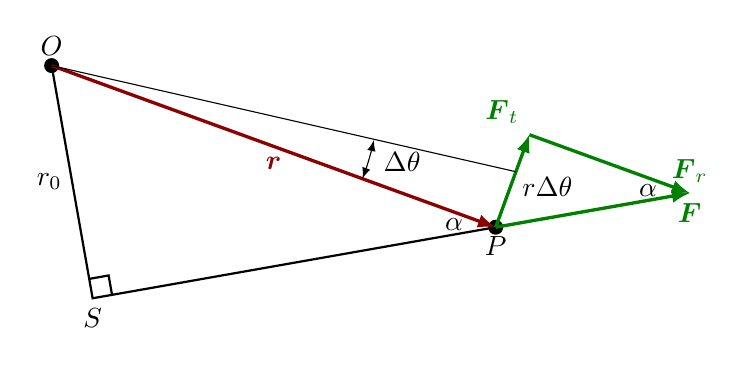
\begin{tikzpicture}[scale=2.5]
  

    
    \pgfmathsetmacro\alp{30} % angle between x and x' axes
    \pgfmathsetmacro\rr{0.1}
    \pgfmathsetmacro\tt{-80}
    \pgfmathsetmacro\r{2.4}
    \pgfmathsetmacro\F{1}
    
    \coordinate (O) at (0,0);
    \coordinate (S) at (\tt:{\r*sin(\alp)});
    \coordinate (P) at ({10-\alp}:\r);
    \coordinate (X) at ({10-\alp}:\r*0.7);
    \coordinate (F) at ($(P) + (10:\F)$); 
    \coordinate (Ft) at ($(P) + ({100-\alp}:{\F*sin(\alp)})$);
    \coordinate (Q) at ($(P) + ({100-\alp}:{\F*sin(\alp)*0.6})$);
    
    \filldraw[] (O) circle (1pt) node [above] {$O$};
    \filldraw[] (P) circle (1pt) node [below] {$P$};
    \draw[thick] (O) -- node[left] {$r_0$} (S) node [below] {$S$}-- (P);
    \draw[thick] ($(S) +({-\tt+20}:\rr)$) --++ (10:\rr) --++ (-80:\rr) ;
    
    \draw[-latex, very thick, mydarkred] (O) -- node [below] {$\boldsymbol{r}$} (P);
    \draw[-latex, very thick, mydarkgreen] (P) -- (F) node[below] {$\boldsymbol{F}$};
    \draw[-latex, very thick, mydarkgreen] (P) -- (Ft) node[above left] {$\boldsymbol{F}_t$};
    \draw[-latex, very thick, mydarkgreen] (Ft) -- (F) node[above ] {$\boldsymbol{F}_r$};
    \draw[] (O) -- (Q);
    %\node[above] at (X) {$\Delta \theta$};
    \node [xshift=-15, yshift=1] at (P) {$\alpha$};
    \node [xshift=-15, yshift=1] at (F) {$\alpha$};
    \node [right, yshift=-2] at ($(P)!0.5!(Ft)$) {$r\Delta \theta$};
    \draw [<->] ($(O)!0.7!(P)$) arc ({10-\alp}:{17-\alp}:0.7*\r) node [yshift=-8, right]{$\Delta \theta$};
\end{tikzpicture}


\end{document}